\documentclass[../DS04.tex]{subfiles}
\graphicspath{{./figures/}}
\addto\captionsfrench{\renewcommand{\figurename}{Fig.}}

% \subimport{/home/nora/Documents/Enseignement/Prepa/bpep/exercices/DS/cinetique_Br2/}{sujet.tex}

\begin{document}

\section[52]"P"{Suivi cinétique de la formation du dibrome\ifcorrige{~\small\textit{(D'après CCMP MP 2012)}}}%

\enonce{%
	À température ambiante, le dibrome de formule \ce{Br2} est un liquide
	brun-orangé très volatil, dégageant des vapeurs toxiques de même couleur.
}

\QR[2]{%
	Justifier la couleur du dibrome en vous servant de son spectre d'absorption,
	donné ci-après.
	\smallbreak
	\noindent
	\begin{isd}[lefthand ratio=.55]
		\begin{center}
			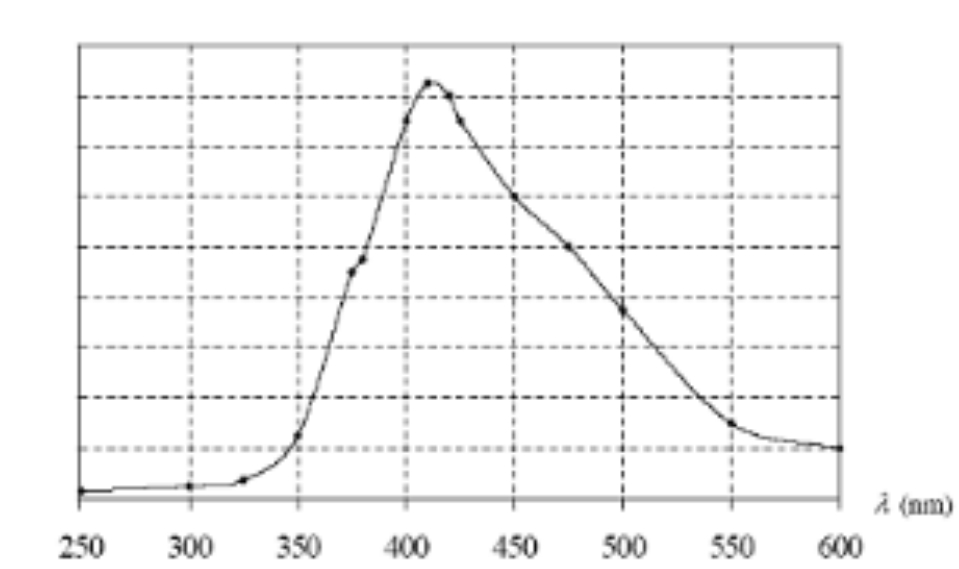
\includegraphics[scale=1]{absorption}
			\captionof{figure}{Spectre d'absorption du dibrome gazeux.}
		\end{center}
		\tcblower
		\begin{center}
			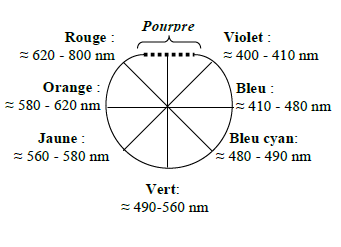
\includegraphics[width=.8\linewidth]{couleur}
			\captionof{figure}{Cercle chromatique simplifié.}
		\end{center}
	\end{isd}
}{%
	Le dibrome absorbe fortement à la longueur d'onde
	$\lambda\approx\SI{400}{\nano\meter}$ \pt{1}. Sa couleur correspond à la couleur
	complémentaire du bleu, soit l'orange \pt{1}.
}

\enonce{%
On effectue la synthèse du dibrome en mélangeant un même volume $V$ d'une
solution de bromate de sodium (\ce{NaBrO3}) de concentration $C_{01} =
	\SI{2,0e-3}{mol.L^{-1}}$ et d'une solution de bromure de sodium (\ce{NaBr}) de
concentration $C_{02} = \SI{1,0e-2}{mol.L^{-1}}$. Des ions
$\ce{H_3O^+_{\aqu}}$ sont naturellement présents en solution. Une coloration
brune apparaît alors après un certain temps.
\bigbreak
L'équation de la réaction est la suivante~:
\begin{gather*}
	\ce{BrO^-_3(aq) + 5 Br^-(aq) + 6H3O+(aq) = 3Br2(aq) + 9H2O(l)}
	\tag{I}
	\label{eq:I}
\end{gather*}
}

\QR[8]{%
	Faire un schéma de la préparation. Cette réaction est réalisée dans des
	conditions où on constate que 90\% des ions bromate ont réagi une fois
	l'équilibre atteint. Déterminer les concentrations des différentes espèces
	bromées à l'équilibre.
}{%
	\pt{1} pour un schéma qui montre que le volume total est $2V$.
	On détermine alors les concentrations initiales $C_1$ et $C_2$ en faisant
	attention au facteur de dilution~:
	\[
		C_1 = \frac{C_{01}}{2} = \SI{1,0e-3}{mol.L^{-1}}
		\stm{\qet}
		C_2 = \frac{C_{02}}{2} = \SI{5,0e-3}{mol.L^{-1}}
	\]
	On effectue un tableau d'avancement en concentration~:
	\begin{center}
		\def\rhgt{0.50}
		\centering
		\begin{tabularx}{\linewidth}{|l|c||YdYdYdYdY|}
			\hline
			\multicolumn{2}{|c||}{
				$\xmathstrut{\rhgt}$
			\textbf{Équation}} \pt{1}+\pt{1} &
			$\ce{BrO^-_3_{\aqu}}$            & $+$         &
			$5\ce{Br^-_{\aqu}}$              & $+$         &
			$6\ce{H_3O^+_{\aqu}}$            & $=$         &
			$3\ce{Br_2_{\aqu}}$              & $+$         &
			$9\ce{H_2O_{\liq}}$
			\\
			\hline
			$\xmathstrut{\rhgt}$
			Initial                          & $x = 0$     &
			$C_1$                            & \vline      &
			$C_2$                            & \vline      &
			$C_3$                            & \vline      &
			$0$                              & \vline      &
			excès
			\tikzmark{MD}                                    \\
			\hline
			$\xmathstrut{\rhgt}$
			Interm.                          & $x\ind{eq}$ &
			$C_1 - x\ind{eq}$                & \vline      &
			$C_2 - 5x\ind{eq}$               & \vline      &
			$C_3 - 6x\ind{eq}$               & \vline      &
			$3x\ind{eq}$                     & \vline      &
			excès
			\tikzmark{ME}                                    \\
			\hline
			% $\xmathstrut{\rhgt}$
			% Final              & $x_f = x_{\equ}$         &
			% $C_1 - x_{}$     & \vline              &
			% $C_2 - 5x_{}$     & \vline              &
			% $0 + 3x_{}$     & \vline              &
			% excès                           \\
			% \hline
		\end{tabularx}
	\end{center}
	\tikz[remember picture, overlay]
	\node[above right=-8pt and 35pt of pic cs:MD] {\pt{1}};
	\tikz[remember picture, overlay]
	\node[above right=-8pt and 35pt of pic cs:ME] {\pt{1}};

	D'après l'énoncé, 90\% des ions \ce{BrO^-_3} ont réagi, donc $x\ind{eq} =
		0,9C_1 = \SI{9,0e-4}{mol.L^{-1}}$. \pt{1} On en déduit les concentrations à
	l'équilibre \pt{1}~:
	\[
		\xul{[\ce{BrO^-_3}]\ind{eq} = \SI{1,0e-4}{mol.L^{-1}}}
		\quad ;\quad
		\xul{[\ce{Br-}]\ind{eq} = \SI{5,0e-4}{mol.L^{-1}}}
		\quad ;\quad
		\xul{[\ce{Br2}]\ind{eq} = \SI{2,7e-3}{mol.L^{-1}}}
	\]
}

\enonce{%
L'étude cinétique de la réaction~\eqref{eq:I} montre que la réaction admet un
ordre vis-à-vis de chacun des réactifs. On se propose de déterminer les ordres
partiels de réaction ainsi que la constante de vitesse.
\bigbreak
On notera respectivement $p$, $q$ et $r$ les ordres partiels des espèces
\ce{BrO^-_{3(aq)}}, \ce{Br^-_{(aq)}} et \ce{H3O+}, et $k$ la constante de
vitesse de la réaction. On considérera que les ordres restent inchangés tout au
long de la réaction.
\bigbreak
Une première expérience est réalisée à $\SI{0}{\degreeCelsius}$ à partir des
concentrations initiales suivantes~:
\[
	[\ce{BrO^-_3}]_0=\SI{1,0e-3}{mol.L^{-1}}
	\quad ;\quad
	[\ce{Br-}]_0 = \SI{1,4e-1}{mol.L^{-1}}
	\quad ;\quad
	[\ce{H3O+}]_0 =\SI{1,0e-1}{mol.L^{-1}}
\]
% L'évolution de la concentration en ions \ce{BrO3-} (que l'on notera $C$ par
% commodité) en fonction du temps est représentée sur la figure~\ref{fig:C}.

% \figCap{0.7}{figC}{Évolution de la concentration en ions bromate (\si{mmol.L^{-1}}) en fonction du temps (\SI{1e3}{\second})\protect\label{fig:C}}
}

\QR[6]{\label{q:kapp}%
	Exprimer la vitesse volumique de la réaction en fonction des concentrations des
	espèces considérées, des ordres partiels et de la constante de vitesse.
	Commenter les concentrations choisies pour réaliser cette expérience. Quelle
	approximation peut-on effectuer~? Comment s'appelle cette méthode~? Sous quelle
	forme peut-on simplifier l'expression de la vitesse volumique de la réaction
	donnée à la question précédente~?
}{\label{q:kapp}%
	\leavevmode\vspace*{-15pt}\relax
	\[
		v \stm{=} k[\ce{BrO^-_3}]^p(t) \cdot [\ce{Br-}]^q(t) \cdot [\ce{H3O+}]^r(t)
	\]
	On constate que $[\ce{H3O+}]_0 \gg [\ce{BrO^-_3}]_0$ et $[\ce{Br-}]_0 \gg
		[\ce{BrO^-_3}]_0$. \pt{1} On peut négliger la variation temporelle de la
	concentration en ions oxonium ainsi que celle en ions bromure. \pt{1} C'est la
	méthode de la dégénérescence de l'ordre. \pt{1}
	Dans ces conditions, la loi de vitesse se simplifie~:
	\[
		\boxed{%
			v \approx
			k[ \ce{Br-}]_0^q\cdot [\ce{H3O+}]_0^r\cdot [\ce{BrO^-_3}]^p \stm{=}
			k\ind{app}[\ce{BrO^-_3}]^p
		}
		\qav
		\boxed{k\ind{app} \stm{=} k [\ce{Br^-}]_0^q \cdot [\ce{H_3O^+}]_0^r}
	\]
}

\QR[13]{%
	Établir les expressions reliant la concentration en ions bromate,
	\textbf{notée $C(t)$ par commodité}, et le temps dans le cas où la réaction
	est d'ordre 0, 1 et 2 par rapport aux ions bromates. Indiquer pour chaque cas
	la régression linéaire à effectuer pour vérifier chaque hypothèse.
}{%
	\leftcenters{%
		Dans chaque cas, la vitesse de la réaction s'écrit
	}{%
		$\DS v(t) \stm{=} - \frac{1}{1} \dv{C}{t}$
	}%
	\vspace{-15pt}
	\smallbreak
	\noindent
	\begin{isd}
		\begin{itemize}
			\item[b]{Ordre 0}~:
			      \begin{DispWithArrows*}
				      v(t) & \stm{=} k\ind{app} C(t)^0
				      \\\Lra
				      \dv{C}{t} & = - k\ind{app}
				      \Arrow{$\DS \int_{0}^{t}$}
				      \\\Lra
				      \Aboxed{C(t) & \stm{=} C_0 - k\ind{app}t}
			      \end{DispWithArrows*}
			      On trace donc
			      \[
				      y\tikzmark{yn0} \stm{=}
				      a\tikzmark{an0}x\tikzmark{xn0} + b\tikzmark{bn0}
			      \]
			      \tikz[remember picture, overlay]
			      \draw[-stealth, transform canvas={xshift=-6pt, yshift=-6pt}]
			      (pic cs:yn0) --++ (-20pt,-10pt)
			      node[anchor=north] {$C(t)$}
			      ; \tikz[remember picture, overlay]
			      \draw[-stealth, transform canvas={xshift=-5pt, yshift=-6pt}]
			      (pic cs:an0) --++(-5pt,-10pt)
			      node[anchor=north] {$-k\ind{app}$}
			      ; \tikz[remember picture, overlay]
			      \draw[-stealth, transform canvas={xshift=0pt, yshift=-6pt}]
			      (pic cs:xn0) --++(10pt,-10pt)
			      node[anchor=north] {$t$}
			      ; \tikz[remember picture, overlay]
			      \draw[-stealth, transform canvas={xshift=3pt, yshift=-6pt}]
			      (pic cs:bn0) --++(10pt,-10pt)
			      node[anchor=north] {$C_0$}
			      ;
			      \vspace{20pt}
		\end{itemize}
		\tcblower
		\begin{itemize}
			\item[b]{Ordre 1}~:
			      \begin{DispWithArrows*}
				      v(t) & \stm{=} k\ind{app} C(t)^1
				      \\\Lra
				      \dv{C}{t} & = - k\ind{app} C(t)
				      \Arrow{$C(t) \stm{=} K\exr^{rt}$\\$C(0) = C_0$}
				      \\\Lra
				      \Aboxed{C(t) & \stm{=} C_0 \exr^{- k\ind{app}t}}
			      \end{DispWithArrows*}
			      On trace donc
			      \[
				      y\tikzmark{yn1} \stm{=}
				      a\tikzmark{an1}x\tikzmark{xn1} + b\tikzmark{bn1}
			      \]
			      \tikz[remember picture, overlay]
			      \draw[-stealth, transform canvas={xshift=-6pt, yshift=-6pt}]
			      (pic cs:yn1) --++ (-20pt,-10pt)
			      node[anchor=north] {$\ln (C(t))$}
			      ; \tikz[remember picture, overlay]
			      \draw[-stealth, transform canvas={xshift=-5pt, yshift=-6pt}]
			      (pic cs:an1) --++(-5pt,-10pt)
			      node[anchor=north] {$-k\ind{app}$}
			      ; \tikz[remember picture, overlay]
			      \draw[-stealth, transform canvas={xshift=0pt, yshift=-6pt}]
			      (pic cs:xn1) --++(10pt,-10pt)
			      node[anchor=north] {$t$}
			      ; \tikz[remember picture, overlay]
			      \draw[-stealth, transform canvas={xshift=3pt, yshift=-6pt}]
			      (pic cs:bn1) --++(10pt,-10pt)
			      node[anchor=north] {$\ln (C_0)$}
			      ;
			      \vspace{20pt}
		\end{itemize}
	\end{isd}
	\begin{isd}
		\begin{itemize}
			\item[b]{Ordre 2}~:
			      \begin{DispWithArrows*}
				      v(t) &\stm{=} k\ind{app} C(t)^2
				      \\\Lra
				      \dv{C}{t} &= - k\ind{app} C(t)^2
				      \\\Lra
				      - \frac{\dd{C}}{C^2} &\stm{=} k\ind{app}
				      \dd{t}
				      \Arrow{$\DS \int_{0}^{t}$}
				      \\\Lra
				      \int_{C_0}^{C}
				      -\frac{\dd{C}}{C^2}
				      &=
				      \int_{t=0}^{t} k\ind{app} \dd{t}
			      \end{DispWithArrows*}
		\end{itemize}
		Or, $\DS \dd\left( \frac{1}{f} \right) \stm{=} - \frac{\dd{f}}{f^2}$~:
		\tcblower
		\begin{DispWithArrows*}[fleqn, mathindent=0pt]
			\Lra
			\int_{C_0}^{C(t)}
			\dd{\left( \frac{1}{C(t)} \right)}
			&=
			k\ind{app} \cdot \int_{t=0}^{t} \dd{t}
			\Arrow{$\DS\int_a^b \dd{(\cdot )} = [(\cdot )]_a^b$}
			\\\Lra
			\frac{1}{C} - \frac{1}{C_0} &=
			k\ind{app} \cdot t
			\\\Lra
			\Aboxed{%
				\frac{1}{C} &\stm{=}
				\frac{1}{C_0} + k\ind{app}t
			}
		\end{DispWithArrows*}
		On trace donc
		\[
			y\tikzmark{yn2} \stm{=}
			a\tikzmark{an2}x\tikzmark{xn2} + b\tikzmark{bn2}
		\]
		\tikz[remember picture, overlay]
		\draw[-stealth, transform canvas={xshift=-6pt, yshift=-6pt}]
		(pic cs:yn2) --++ (-20pt,-10pt)
		node[anchor=north] {$\frac{1}{C}$}
		; \tikz[remember picture, overlay]
		\draw[-stealth, transform canvas={xshift=-5pt, yshift=-6pt}]
		(pic cs:an2) --++(-5pt,-10pt)
		node[anchor=north] {$k\ind{app}$}
		; \tikz[remember picture, overlay]
		\draw[-stealth, transform canvas={xshift=0pt, yshift=-6pt}]
		(pic cs:xn2) --++(10pt,-10pt)
		node[anchor=north] {$t$}
		; \tikz[remember picture, overlay]
		\draw[-stealth, transform canvas={xshift=3pt, yshift=-6pt}]
		(pic cs:bn2) --++(10pt,-10pt)
		node[anchor=north] {$\frac{1}{C_0}$}
		;
		\vspace{20pt}
	\end{isd}
	\vspace{-15pt}
}%

\enonce{%
	On a relevé les données suivantes (Tableau~\ref{tab:data}) de la concentration en
	ions $\ce{BrO_3-}$, notée $C$ par commodité, en fonction du temps~:
	\begin{table}[htbp!]
		\centering
		\caption{Données de $c(t)$}
		\begin{tabular}{cccccccc}
			\toprule
			$t$ (\si{s})              &
			\num{0}                   &
			\num{2.0}                 &
			\num{3.5}                 &
			\num{5.0}                 &
			\num{10.0}                &
			\num{19.0}                &
			\num{38.5}
			\\
			\midrule
			$C(t)~(\si{mmol.L^{-1}})$ &
			\num{1.00}                &
			\num{0.93}                &
			\num{0.88}                &
			\num{0.83}                &
			\num{0.69}                &
			\num{0.50}                &
			\num{0.25}
			\\
			\bottomrule
		\end{tabular}
		\label{tab:data}
	\end{table}
}%

\QR[9]{%
	Tracer chaque régression sur votre calculatrice et reproduire sommairement
	l'allure des courbes sur votre copie. Vous prendrez soin d'indiquer l'unité
	des axes pour chacun d'eux. En déduire l'ordre partiel de la réaction par
	rapport aux ions bromate. Justifier. Déterminer alors la constante de vitesse
	apparente.
}{%
	On obtient
	\smallbreak
	\noindent
	\begin{minipage}[c]{.32\linewidth}
		\begin{center}
			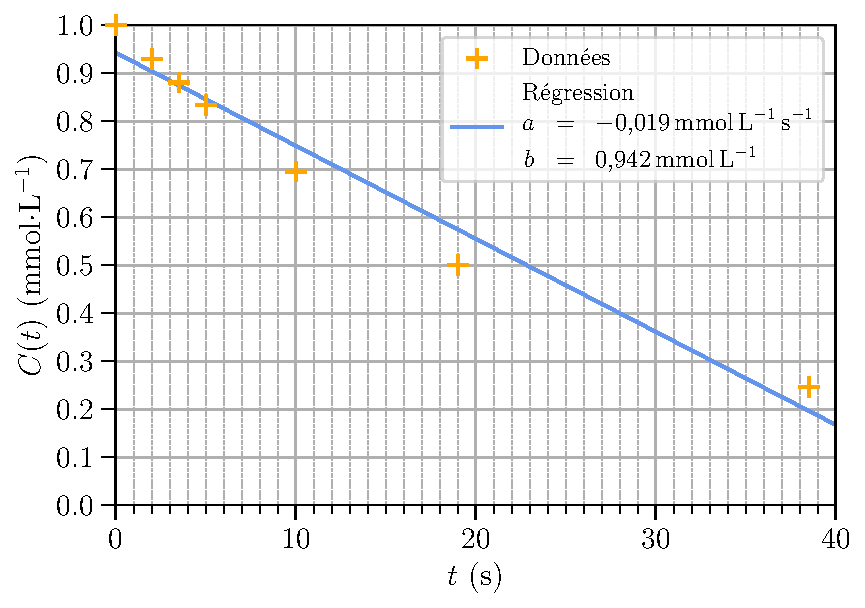
\includegraphics[width=\linewidth]{c(t)}
			\captionof{figure}{Régression ordre 0. \protect\pt{2}}
		\end{center}
	\end{minipage}
	\hfill
	\begin{minipage}[c]{.32\linewidth}
		\begin{center}
			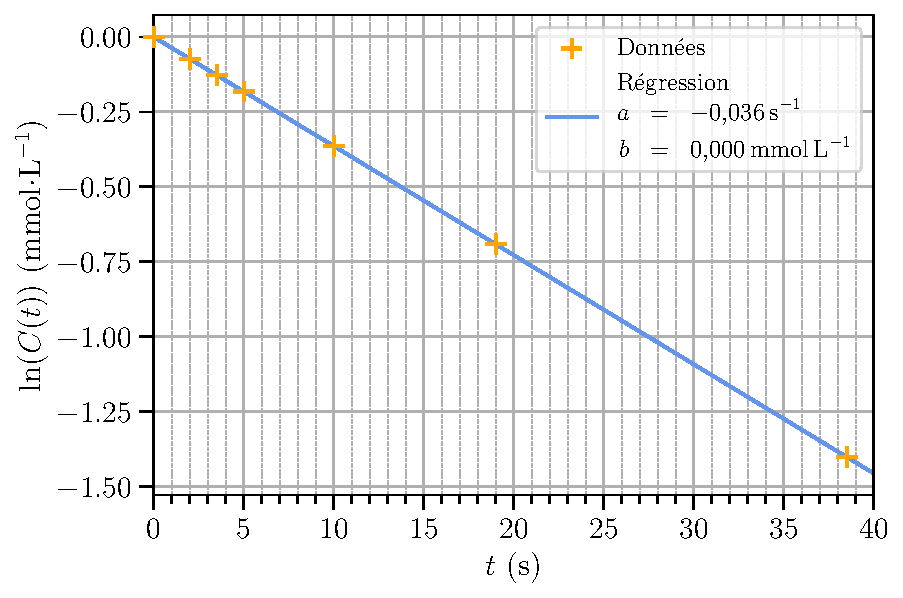
\includegraphics[width=\linewidth]{lnc(t)}
			\captionof{figure}{Régression ordre 1. \protect\pt{2}}
			\label{fig:lnC}
		\end{center}
	\end{minipage}
	\hfill
	\begin{minipage}[c]{.32\linewidth}
		\begin{center}
			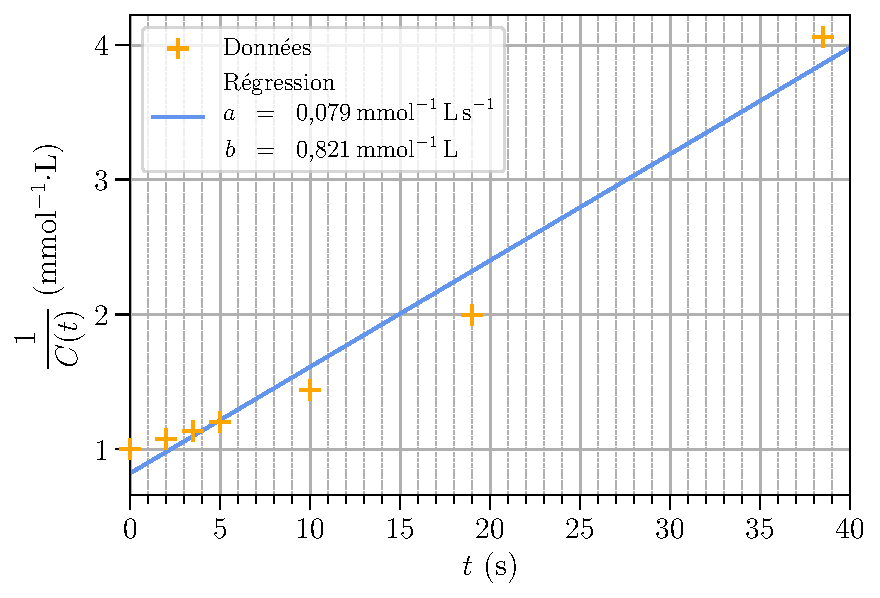
\includegraphics[width=\linewidth]{invc(t)}
			\captionof{figure}{Régression ordre 2. \protect\pt{2}}
		\end{center}
	\end{minipage}
	\bigbreak
	La seule régression valide est celle de la Figure~\ref{fig:lnC}, puisque la
	droite passe effectivement par les points sans déviation particulière \pt{1}~:
	on a donc
	\[
		\xul{p = 1} \pt{1}
	\]
	De plus, d'après la régression linéaire établie précédemment, on obtient
	\[
		a = -k\ind{app}
		\Ra
		\xul{k\ind{app} = \SI{3.6e-2}{s^{-1}}} \pt{1}
	\]
}%

\QR[2]{%
	Définir et déterminer ensuite le temps de demi-réaction relatif aux ions
	bromate.
}{%
	Par définition, on a $t_{1/2}$ tel que
	\[
		\boxed{C(t_{1/2}) \stm{=} \frac{C(0)}{2}}
	\]
	Ici, avec $C(0) = \SI{1.0}{mmol.L^{-1}}$, on trouve $C(t_{1/2}) =
		\SI{0.50}{mmol.L^{-1}}$, et on a donc directement $t_{1/2}$ dans
	le Tableau~\ref{tab:data}~:
	\[
		\xul{t_{1/2} = \SI{19}{s}} \pt{1}
	\]
}%

\enonce{%
	Plusieurs autres expériences ont été réalisées à $\SI{0}{\degreeCelsius}$ pour
	une même concentration initiale en ions bromate $[\ce{BrO3-}]_0
		=\SI{1,0e-3}{mol.L^{-1}}$ et pour des concentrations variables en ions bromure
	et oxonium. Dans chaque expérience, la vitesse initiale a été déterminée. Les
	résultats sont rassemblés dans le tableau suivant~:
	\begin{center}
		\begin{tabular}{|c|c|c|c|}
			\hline
			Expériences                      &
			$[\ce{Br-}]_0(\si{mol.L^{-1}})$  &
			$[\ce{H3O+}]_0(\si{mol.L^{-1}})$ &
			Vitesse initiale $(\si{\mole\cdot \liter^{-1}\cdot\second^{-1}})$
			\\\hline
			N°1                              &
			\num{0,10}                       &
			\num{0,10}                       &
			\num{4.1e-5}
			\\
			\hline
			N°2                              &
			\num{0,15}                       &
			\num{0,10}                       &
			\num{6.2e-5}
			\\
			\hline
			N°3                              &
			\num{0,10}                       &
			\num{0,20}                       &
			\num{16.4e-5}
			\\
			\hline
		\end{tabular}
	\end{center}
}

\QR[9]{%
	Déterminer l'ordre partiel par rapport aux ions bromures et l'ordre partiel
	par rapport aux ions \ce{H3O+}.
}{%
	On pose le système d'équations~:
	\begin{eqnarray}
		v_{01} &=
		k [\ce{BrO^-_3}]_0 \cdot [\ce{Br^-}]_{01}^q \cdot [\ce{H_3O^+}]_{01}^r
		\label{eq:1}
		\\
		\pt{1} \quad
		v_{02} &=
		k [\ce{BrO^-_3}]_0 \cdot [\ce{Br^-}]_{02}^q \cdot [\ce{H_3O^+}]_{02}^r
		\label{eq:2}
		\\
		v_{03} &=
		k [\ce{BrO^-_3}]_0 \cdot [\ce{Br^-}]_{03}^q \cdot [\ce{H_3O^+}]_{03}^r
		\label{eq:3}
	\end{eqnarray}
	\begin{isd}
		\begin{align*}
			\eqref{eq:2} / \eqref{eq:1}
			\Ra
			\frac{v_{02}}{v_{01}} & \stm{=}
			\left( \frac{[\ce{Br^-}]_{02}}{[\ce{Br^-}]_{01}} \right)^q
			\\\qcar
			[\ce{H_3O^+}]_{02}    & \stm{=}{} [\ce{H_3O^+}]_{01}
			\\\Lra
			\Aboxed{%
			q                     & \stm{=}
				\frac{\ln (v_{02}/v_{01})}{\ln ([\ce{Br^-}]_{02}/[\ce{Br^-}]_{01})}
			}
			\\\AN
			\makebox[0pt][l]{$\xul{\phantom{q = 1}}$}
			q                     & = 1
			\quad \pt{1}
		\end{align*}
		\tcblower
		\begin{align*}
			\eqref{eq:3} / \eqref{eq:1}
			\Ra
			\frac{v_{03}}{v_{01}} & \stm{=}
			\left( \frac{[\ce{H_3O^+}]_{03}}{[\ce{H_3O^+}]_{01}} \right)^r
			\\\qcar
			[\ce{Br^-}]_{03}      & \stm{=}{} [\ce{Br^-}]_{01}
			\\\Lra
			\Aboxed{%
			r                     & \stm{=}
				\frac{\ln (v_{03}/v_{01})}{\ln ([\ce{H_3O^+}]_{03}/[\ce{H_3O^+}]_{01})}
			}
			\\\AN
			\makebox[0pt][l]{$\xul{\phantom{b = 1}}$}
			r                     & = 1
			\quad \pt{1}
		\end{align*}
	\end{isd}
	% \begin{itemize}
	% 	\item[m]
	% 	      \begin{align*}
	% 		      \eqref{eq:2} / \eqref{eq:1}
	% 		      \Ra
	% 		      \frac{v_{02}}{v_{01}} & \stm{=}
	% 		      \left( \frac{[\ce{Br^-}]_{02}}{[\ce{Br^-}]_{01}} \right)^q
	% 		      \qcar
	% 		      [\ce{H_3O^+}]_{02} \stm{=}{} [\ce{H_3O^+}]_{01}
	% 		      \\\Lra
	% 		      \Aboxed{%
	% 		      q                     & \stm{=}
	% 			      \frac{\ln (v_{02}/v_{01})}{\ln ([\ce{Br^-}]_{02}/[\ce{Br^-}]_{01})}
	% 		      }
	% 		      \qav
	% 		      \left\{
	% 		      \begin{array}{rcl}
	% 			      v_{01}           & = & \SI{4.1e-5}{mol.L.s^{-1}}
	% 			      \\
	% 			      v_{02}           & = & \SI{6.2e-5}{mol.L.s^{-1}}
	% 			      \\{}
	% 			      [\ce{Br^-}]_{01} & = & \SI{0.10}{mol.L^{-1}}
	% 			      \\{}
	% 			      [\ce{Br^-}]_{02} & = & \SI{0.15}{mol.L^{-1}}
	% 		      \end{array}
	% 		      \right.                         \\
	% 		      \AN
	% 		      \makebox[0pt][l]{$\xul{\phantom{q = 1}}$}
	% 		      q                     & = 1
	% 		      \quad \pt{1}
	% 	      \end{align*}
	% 	\item[m]
	% 	      \begin{align*}
	% 		      \eqref{eq:3} / \eqref{eq:1}
	% 		      \Ra
	% 		      \frac{v_{03}}{v_{01}} & \stm{=}
	% 		      \left( \frac{[\ce{H_3O^+}]_{03}}{[\ce{H_3O^+}]_{01}} \right)^r
	% 		      \qcar
	% 		      [\ce{Br^-}]_{03} \stm{=}{} [\ce{Br^-}]_{01}
	% 		      \\\Lra
	% 		      \Aboxed{%
	% 		      r                     & \stm{=}
	% 			      \frac{\ln (v_{03}/v_{01})}{\ln ([\ce{H_3O^+}]_{03}/[\ce{H_3O^+}]_{01})}
	% 		      }
	% 		      \qav
	% 		      \left\{
	% 		      \begin{array}{rcl}
	% 			      v_{01}             & = & \SI{4.1e-5}{mol.L.s^{-1}}
	% 			      \\
	% 			      v_{03}             & = & \SI{6.2e-5}{mol.L.s^{-1}}
	% 			      \\{}
	% 			      [\ce{H_3O^+}]_{01} & = & \SI{0.10}{mol.L^{-1}}
	% 			      \\{}
	% 			      [\ce{H_3O^+}]_{03} & = & \SI{0.15}{mol.L^{-1}}
	% 		      \end{array}
	% 		      \right.                         \\
	% 		      \AN
	% 		      \makebox[0pt][l]{$\xul{\phantom{b = 1}}$}
	% 		      r                     & = 1
	% 		      \quad \pt{1}
	% 	      \end{align*}
	% \end{itemize}
	\vspace{-15pt}
}

\QR[3]{%
	Calculer la constante de vitesse $k$ de la réaction. Préciser clairement son
	unité.
}{%
	D'après~\ref{q:kapp} et en prenant les données de l'expérience
	\textbf{initiale}, on a
	\begin{align*}
		\Aboxed{%
			k \stm{=} \frac{k\ind{app}}{[\ce{Br^-}]_{0}\cdot [\ce{H_3O^+}]_{0}^2}
		}
		\qav
		\left\{
		\begin{array}{rcl}
			k\ind{app}        & =       & \SI{3.6e-2}{s^{-1}}
			\\{}
			[\ce{Br^-}]_{0}   & \stm{=} & \SI{0.14}{mol.L^{-1}}
			\\{}
			[\ce{H_3O^+}]_{0} & =       & \SI{0.10}{mol.L^{-1}}
		\end{array}
		\right.                                          \\
		\AN
		\makebox[0pt][l]{$\xul{\phantom{k \approx \SI{26}{mol^{-3}.L^{3}.s^{-1}}}}$}
		k & \stm{\approx} \SI{26}{mol^{-3}.L^{3}.s^{-1}}
	\end{align*}
}

\end{document}
